\chapter{BACKGROUND KNOWLEDGE}
\label{chap:background}

\paragraph{Chapter 2} Presentation of background knowledge necessary for the implementation process, including the content:

\section{Crowd-sourcing}
\subsection{Definition}
Crowdsourcing is a relatively new approach for knowledge acquisition, information diffusion, the exchange of thoughts and views among experts and the crowd, etc \cite{futureinternet0600109}. Based on this approach, several kinds of problems can be distributed and resolved through the adoption of appropriate web-based platforms designed for such a purpose. The exploitation of collective knowledge and intelligence results in the creation of innovative ideas, where in some cases, participants earn money or gain a “prize” as acknowledgment for their contribution. The advent of the World Wide Web and the spread of the Internet have led to the development of online systems through which people from all over the world have the opportunity to participate in a problem solving process with or without the contribution of experts. 

Therefore, crowdsourcing can be considered as a process evolving through the following steps: the online release of a problem, the generation of alternative solutions by the crowd (participants), the evaluation of the proposed solutions, the selection of the best provided solution and the exploitation of the selected solution by the company or institution that initially posted the problem online.

 Among the most representative crowdsourcing applications that have been developed with the upport of the so-called “crowdsourced” information are Wikipedia, Waze (a free turn-by-turn GPS application for mobile phones that uses crowdsourcing to provide routing and real-time traffic updates), Arcbazar (an American crowdsourcing platform for architectural design services), Facebook (used crowdsourcing to create different language versions of its site) and OSM (OpenStreetMap).
 
  As mentioned above, crowdsourcing is based on the principle that nobody knows everything, as everyone has a share in knowledge. In this context, the “wisdom of the crowd” can be utilized during the problem solving process through the “aggregation” of several proposed solutions \cite{doi101177}. Such a process can be facilitated by the adoption of new web technologies that offer the crucial advantage of “bringing people together”. Different views and perspectives can lead to different solutions, some of which may be unexpectedly remarkable.
  
  
  On the other hand, participants in a crowdsourcing process gain several benefits. They acquire new skills. They perceive the “seeking to the best solution” process as a challenge to achieve, and they also gain new knowledge. In some cases, they can also “incorporate that experience in the seeking of better employment or in the goal of establishing oneself in freelance work as an entrepreneur” \cite{doi101177}. Crowdsourcing is a model appropriate for the utilization of collective talents by aggregating collective intelligence and knowledge and also by increasing the ingenuity of the crowd. This may result in innovative solutions by reducing the cost and time a traditional problem solving process usually requires \cite{doi101177}

\section{Neural network}

\subsection{Artificial Neural Network (ANN)}
The human brain consists of many computational units called neuron. The \textbf{Artificial neural network (ANN)} is vaguely inspired by that structure. An ANN is a collection of connected nodes called the artificial neurons. Each artificial neuron is a computational unit with inputs and an output.
\begin{center}
	\begin{figure}[H]
		\centering
		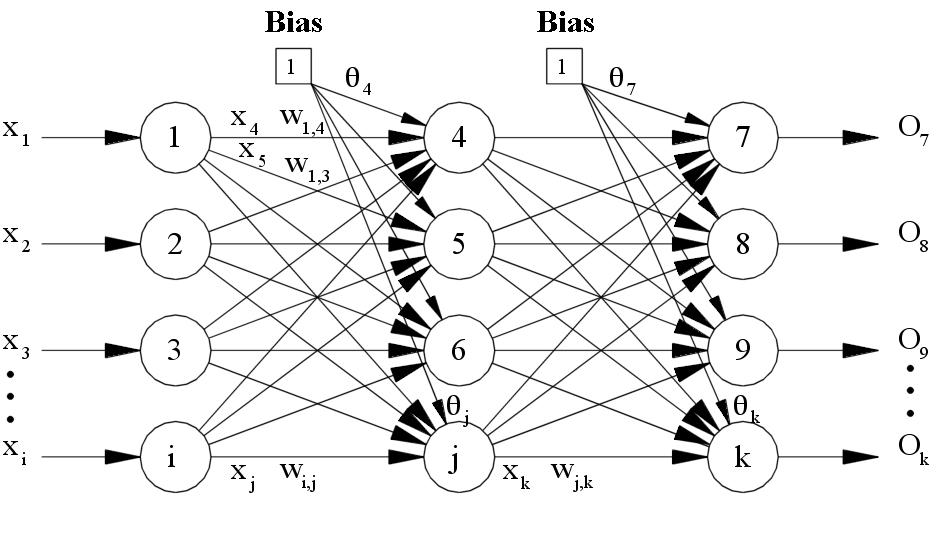
\includegraphics[width=0.75\columnwidth]{images/chap2/NeuralNetwork.jpg}
		\caption{A 2-layer Neural Network (one hidden layer of 4 neurons (or units) and one output layer with 2 neurons), and three inputs.}
		\label{chap2:neural_net}
	\end{figure}
\end{center}
\footnotetext{Source: \url:{ https://devblogs.nvidia.com/mocha-jl-deep-learning-julia/}}

Figure \ref{chap2:neural_net} represents a simple artificial neural network, where each circle is an artificial neuron, inward and outward arrows are the inputs and outputs of that neuron. The first layer where there is no input is called the “input layer”. Similarly, the last layer where there is no output is called the ‘output layer’. Layers that are either input or output are called “hidden layers”. In the figure, every neuron of one layer is connected to all neuron in the next layer, so it every layer is a “fully-connected layer”. A Network which only have Fully-connected layer(s) is also called as Multi Layer Perceptron (MLP). A connection between two artificial neurons is called an ‘edge’. Artificial neurons and edges will have a ‘weight’ value \boldmath$W$ to adjust the learning process. Increasing or decreasing the weight value will affect the strength of the signal between two neurons. A typical artificial neuron will take each input, multiply it with the corresponding weight \boldmath$W$, take the sum of its input and apply some non-linear function (activation function \boldmath$\varphi$ to get the output. Many connections of artificial neuron form a neural network, where the output of a neuron is the input of another artificial neuron. Typically, an artificial neuron network will have many layers. If the weight is set correctly, the ANN can be used to estimate numerous complex mathematical problems.

\begin{center}
	\begin{figure}[H]
		\centering
		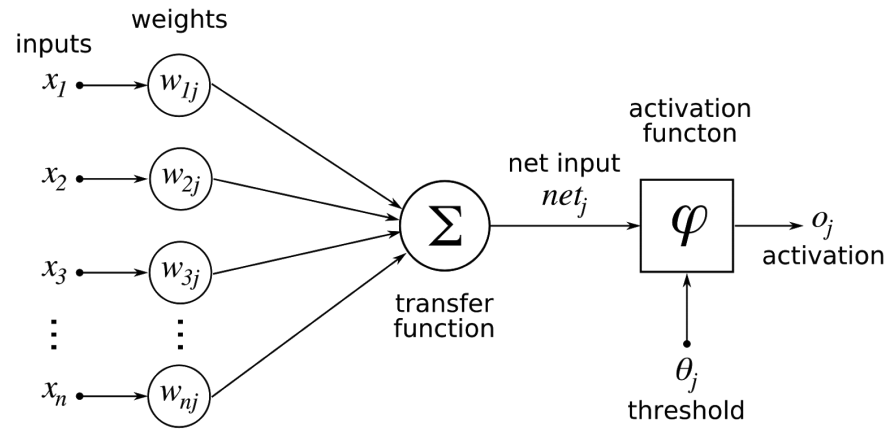
\includegraphics[width=0.75\columnwidth]{images/chap2/ANN_detail.png}
		\caption{Detail of processing in ANN}
		\label{chap2:neural_net_detail}
		
	\end{figure}
\end{center}

\subsection{Activation Function:}
Many non-linear functions can be used with neurons. Currently, there is no theory about the use of non-linear functions in any case, and the selection of suitable nonlinear functions for a particular task in the experiment. In nonlinear functions, the following functions are most commonly used: Tanh, Sigmoid, ReLU
\begin{itemize}
	\item \textbf{Tanh}\\
	Tanh function has a formula:  $\tanh(x) = \frac{e^{2x-1}}{e^{2x+1}}$ has an S-shaped graph, and takes the value of x to [-1,1]
	\begin{center}
		\begin{figure}[H]
			\centering
			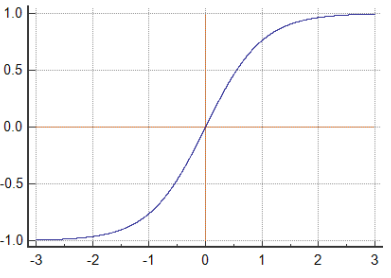
\includegraphics[width=0.5\columnwidth]{images/chap2/tanh.png}
			\caption{Tanh function graph}
			\label{chap2:tanh}
		\end{figure}
	\end{center}
	\item \textbf{Sigmoid}\\
	Sigmoid function has a formula: $ \sigma(x) = \frac{1}{1+\exp e^{-x}}$ has an S-shaped graph, and takes the value of x to [-1,1]
	\begin{center}
		\begin{figure}[H]
			\centering
			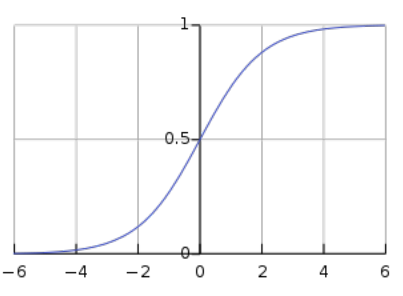
\includegraphics[width=0.5\columnwidth]{images/chap2/sigmoid.png}
			\caption{Sigmoid function graph}
			\label{chap2:sigmoid}
		\end{figure}
	\end{center}
	\item \textbf{ReLU}\\
	Rectified linear Unit is a simple nonlinear function but has very good results in experiments, it's has formula $ReLU(x) = max (0,x)$
		\begin{center}
		\begin{figure}[H]
			\centering
			\includegraphics[width=0.5\columnwidth]{images/chap2/ReLU.png}
			\caption{ReLU function graph}
			\label{chap2:relu}
		\end{figure}
	\end{center}
\end{itemize}

\subsubsection{Softmax}

With classification problems, the \textbf{Output layer} is often a \textbf{Softmax Regression} layer that calculates the probability that a data point falls into each class. Softmax has a simple fomula:\\
\begin{center}
	$ softmax(x) = $\scalebox{1.4}{$\frac{e^{x_{j}}}{\sum\limits_{j=1}^k e^{x_{j}}} $}$, \forall X = [x_{1},x_{2},...x_{k}]$
\end{center}


\begin{center}
	\begin{figure}[H]
		\centering
		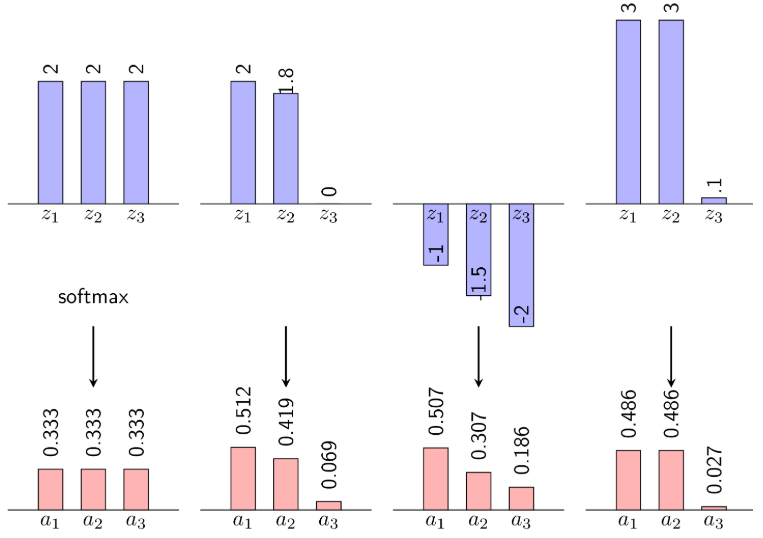
\includegraphics[width=0.75\columnwidth]{images/chap2/Softmax.png}
		\caption{Some examples of Softmax input and output}
		\label{chap2:softmax}
		
	\end{figure}
\end{center}
\subsubsection{Loss function}
When training an artificial neural network, the loss function needs to be defined, L ($\hat{y}, y$) showing the difference between the predicted $\hat{y}$ result and the correct value y. This function always has a non-negative value and is only 0 when $\hat{y}$ equals y.

The normal training process will be to adjust the model parameters (Weight W and bias b) so that the loss function value is as small as possible.

A loss function is any function that takes two vectors and returns a scalar value. For optimization purposes, the loss function is often defined so that it is easy to calculate the derivative

For multi-layer classification, the commonly used loss function is categorical cross-entropy
\textbf{Categorical cross-entropy} is used when expect outputs to be a probability.
With $y$ is one-hot encode vector representing the correct class of input and $\hat{y} = [\hat{y_1},\hat{y_2},..,\hat{y_n}$ is the output vector of the network has been transformed by Softmax function and can be considered as a representation of the first data in class $i: \hat{y} = P(y = i|x)$. Categorical cross-entropy measures the difference between $\hat{y}$ and $y$ distributions
\begin{center}
	$L_{cross-entropy}(\hat{y},\hat{y}) = - \sum\limits_{i}y_{i}\log(\hat{y}_{i})$
\end{center}
\subsection{Convolution Neural Network (CNN)}
\subsubsection{Overview}
The CNN is inspired by the visual nerve system in animals, which is responsible for processing brain imaging data. Within this system, specific neurons only emit signals when a specific feature appear in the visual area. The human brain processes images through each layer with increasing complexity. The first layer distinguishes essential characteristics such as straight lines or curves. On the next layer, the brain will recognize the current arrangement of lines and colors that represent a dog or a cat. Similarly, CNN also processes images using multiple weight matrices called filters to detect features such as edges, lines... When going to higher layers, filters will be able to identify complex properties.

\subsubsection{Convolution Neural Network Architechture}
Simple architecture for Convolution Neural Network could be [INPUT - CONV - RELU - POOL - FC]. In more detail:

\begin{itemize}
	\item Input: [width-heigth-channel] for example in CIFAR -10 classifications, the input is [32x32x3] which hold the raw pixel values of the image, in this case, an image of width 32, height 32, and with three color channels Red, Blue, Green ( [32x32x3])
	\item CONV layer is the most important layer, will compute the output of neurons that are connected to local regions in the input, the returned result could be [32x32x12] if 12 filters are decided to be used 
	\item RELU layer (Rectified linear unit) will apply an elements wise activation function (it is also the most commonly used activation function in deep learning models). The function returns 0 if it receives any negative input, but for any positive value x, it returns x back. F(x) = max(0,x)\\
	\item POOL (Pooling) layer will perform a downsampling operation along the spatial dimensions (Width, Height), result in volume such as [16 x 16 x 12]
	\item FC (Fully-connected) layer will compute the score of classes, resulting in a volume of size [1 x 1 x number of class] in Cifar-10, it returns [1x1x10]
\end{itemize}

By this way, CNN transforms the original image layer by layer from raw pixel values to the final class score. Note that some layers contain parameters, and others do not. For instance, CONV and FC layers contain not only the activation but also weight and the biases of the neurons. On the other hand, the RELU/POOL layers will implement a fixed function. The parameters in the CONV/FC layers will be trained with the gradient descent algorithm so that the class scores that the CNN computes are consistent with the labels in training set for each image.\\

Convolution layer is the core building block of a Convolution Network that does the most critical computations in the Network.
\begin{center}
  \begin{figure}[H]
  \centering
  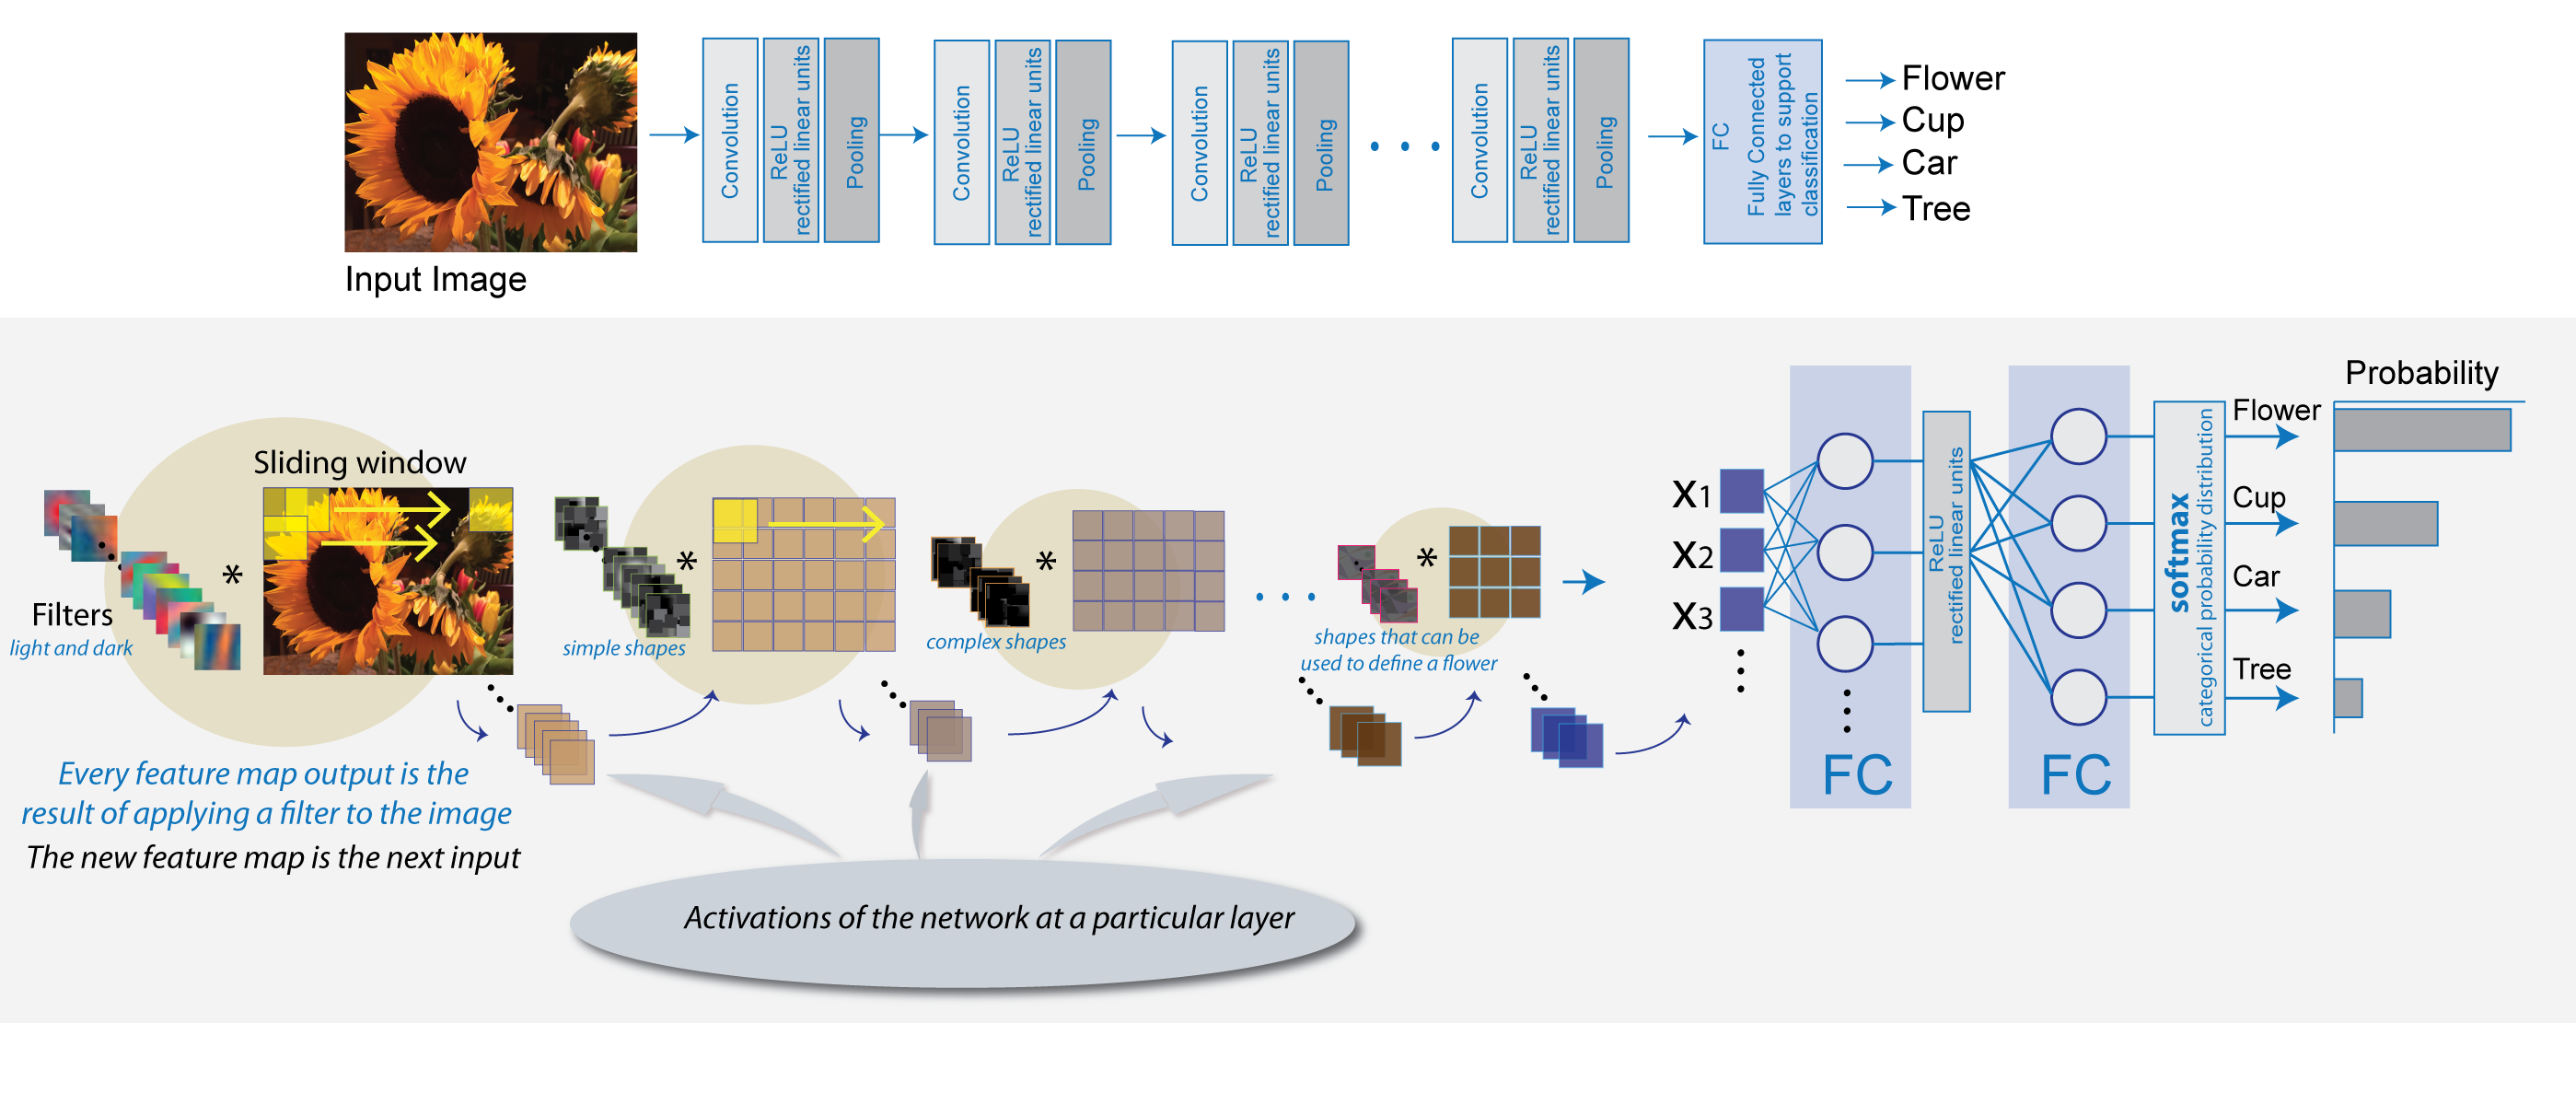
\includegraphics[width=1\columnwidth]{images/chap2/Intro_CNN.png}
  \caption{Simple Convolution Neural Network Architecture}
  \label{chap2:CNN arch}
  \end{figure}
\end{center}

\vspace{-1cm}
\subsubsection{Convolution Layer}
\begin{itemize}
	\item Overview:\\ 
	The convolution layer's parameter consists of a set of learnable filters. Every filter is small spatially [ Width x Height], but extends through the full depth of the input volume (in standard image, the depth is equal 3). For example, a typical filter on the first layer of a CNN might have a size [5x5x3] (5 pixels width and height, and depth = 3). In the calculating process, slide each filter across the width and height of the input and compute dot-product between input and filter in every position. The result of dot-product is a 2-dimensional matrix called activation map of a filter. With layer has 12 filters, each of them produces one activation map, then stack these maps along the depth dimension and produce the output volume.
	\item Local Connectivity:\\
	When processing input which high-dimensional such as images, connect neurons to all previous neurons like Fully-connected layer is impractical, a number of parameters of the network must learn is massive (exploding hyperparameters). Alternately, each neuron is connected to only a local region of the input volume,the limit region of this connectivity is a hyperparameter called receptive field of the neuron (equivalently this is the size of the filter). The connections are local in space (along with width and height), but always full along the entire of the depth of the input volume.
	\begin{center}
		\begin{figure}[H]
			\centering
			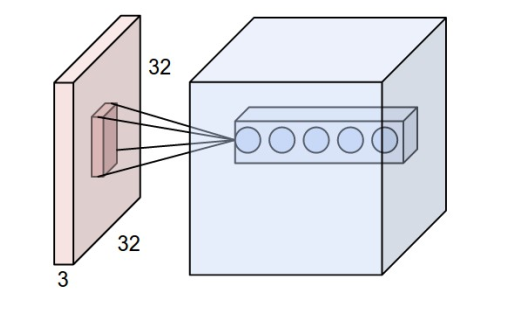
\includegraphics[width=1\columnwidth]{images/chap2/LocalConnectivity.png}
			\caption{Local connectivity in Convolution Neural Network}
			\label{chap2:LocalConnectivity}
		\end{figure}
	\end{center}
	\vspace{-1cm}
	\item Output volume: There is three hyperparameters affect the output volume: the depth, stride, and zero-padding.\\
	\begin{enumerate}
		\item Depth: Depth of output volume is corresponds to the number of filters used in the network. Each filter learning to look for something different in the input. For instance, with input is a raw image. First Conv Layer can learn a way to detect some primary attribute like edge, color or blobs … Set of neurons that are all looking at the same region of the input are called depth column (sometimes called fiber).\\
		\item Stride: stride is the step of filter over input. If stride is 1, a filter is moved 1 pixel per step, identical to stride equal 2 or 3. Therefore, this will produce smaller output volumes spatially ( smaller in Width and Height)
		\item Zero-Padding: Zero-padding is the number of line of Zero around the input volume, applying zero-padding allow us to control Height and Width of output volume (Commonly, it is used to preserve the spatial size of the input and output volume)
		
	\end{enumerate}
\end{itemize}

Output volume can be computed by using input volume size (W), the receptive field size of the Convolution Layer neurons (F), the stride value (S), and the amount of zero padding used (P) on the border. The formula for calculating how many neurons "fit" is given by:
\begin{center}
	\[ \scalebox{1.5}{$\frac{W_{1} - F + 2P }{S} + 1$} \]
\end{center}
For example, with input (W) = 7x7, filter (F) = 3x3, stride (F) = 1, Zero-padding 1, the output will be 5x5




\begin{center}
  \begin{figure}[H]
  \centering
  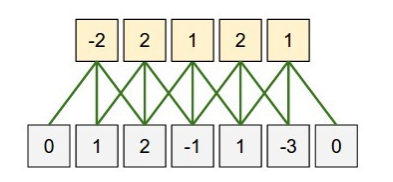
\includegraphics[width=1\columnwidth]{images/chap2/Output_volume_WSP.png}
  \caption{Output volume with F = 3, W = 5, S = 1 and Zero-Padding P = 1 }
  \label{chap2:Outputvolume_example}
  \end{figure}
\end{center}
\textbf{Summary Convolution Layer:}
\begin{itemize}
	\item Accept a volume size $W_{1}$ x $H_{1}$ x $D_{1}$ as input
	\item Requires four hyperparameters:
	\item Number of filter K
	\item Their spatial extent F 
	\item The stride S
	\item The amount of zero padding P
	\item Return an output with volume $W_{2}$ x $H_{2}$ x $D_{2}$ with:
	\begin{align*}
		W_{2} &= \frac{W_{1} - F + 2P }{S} + 1 \\
		H_{2} &= \frac{H_{1} - F + 2P }{S} + 1 \\
		D_{2} &= K
	\end{align*}
\end{itemize}

\subsubsection{Pooling Layer:}
Pooling Layer's function is to progressively reduce the spatial size of the representation to reduce the number of parameters and computation in the network, and control overfitting too. Pooling Layer operates independently on every depth slice of the input and resizes it spatially, using MAX, AVERAGE, SUM operation. The most common form is a pooling with MAX operation, filters of size 2x2 applied with a stride of 2, it will downsample every depth slice in the input by two along both width and height (depth is remaining).\\
\begin{center}
  \begin{figure}[H]
  \centering
  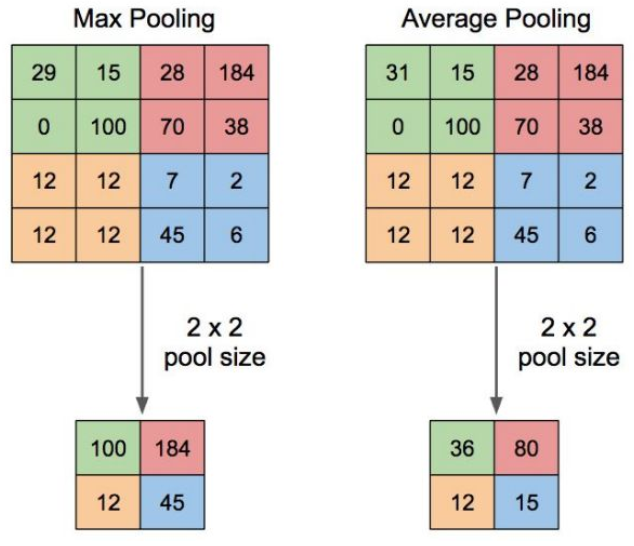
\includegraphics[width=1\columnwidth]{images/chap2/Pooling.png}
  \caption{Max Pooling and Average Pooling}
  \label{chap2:MaxPooling and Average Polling}
  \end{figure}
\end{center}

\textbf{Summary Pooling layer:}
\begin{itemize}
	\item Accept a volume size $W_{1}$ x $H_{1}$ x $D_{1}$ as input
	\item Require two hyperparameters:
	\item Their spatial extent F 
	\item The stride S
	\item Produces a volume of size $W_{2}$ x $H_{2}$ x $D_{2}$ with:
	\begin{align*}
	W_{2} &= \frac{W_{1} - F }{S} + 1\\
	H_{2} &= \frac{H_{1} - F }{S} + 1\\
	D_{2} &= D_{1}
	\end{align*}
	\item No parameter, because it computes a fixed function of the input\\
	\item Zero-Padding is unusable in pooling layer
\end{itemize}



\subsubsection{Fully-Connected Layer:}
Same as Fully Connected in ANN, neurons in a fully connected layer have full connections to all activation functions in the previous layer. 

\subsubsection{Some well-known CNN architecture:}
\textbf{LeNet (1998):} Yann LeCun developed LeNet first successful applications of Convolutional Network in the 1990s. LeNet is used to reading zip code, digits.
\begin{center}
  \begin{figure}[H]
  \centering
  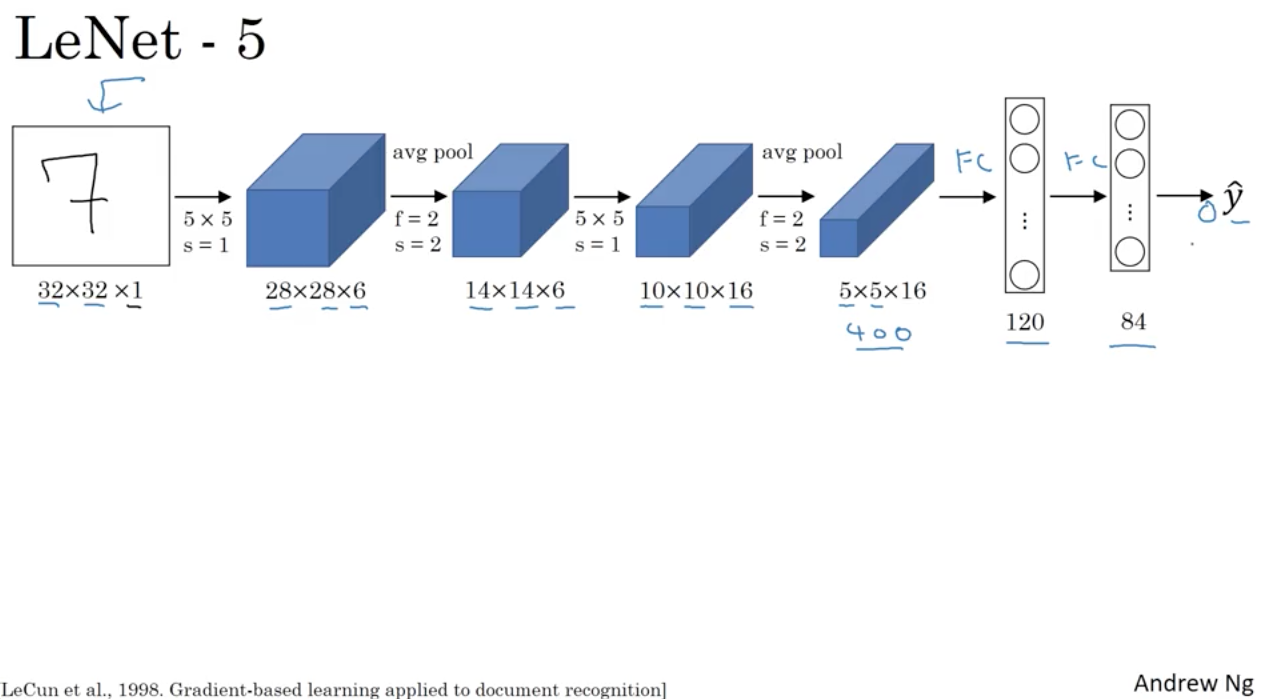
\includegraphics[width=1\columnwidth]{images/chap2/LeNet.png}
  \caption{LeNet Architecture}
  \label{chap2:WSP}
  \end{figure}
\end{center}
\textbf{AlexNet (2012):} The first work that popularized Convolutional Networks in Computer Vision was the AlexNEt, developed by Alex Krizhevsky. The AlexNet got the first prize in ImageNet ILSVRC challenge 2012 and significantly outperformed the second (top 5 error of 16\% compared to runner-up with 26\% error).  
\begin{center}
  \begin{figure}[H]
  \centering
  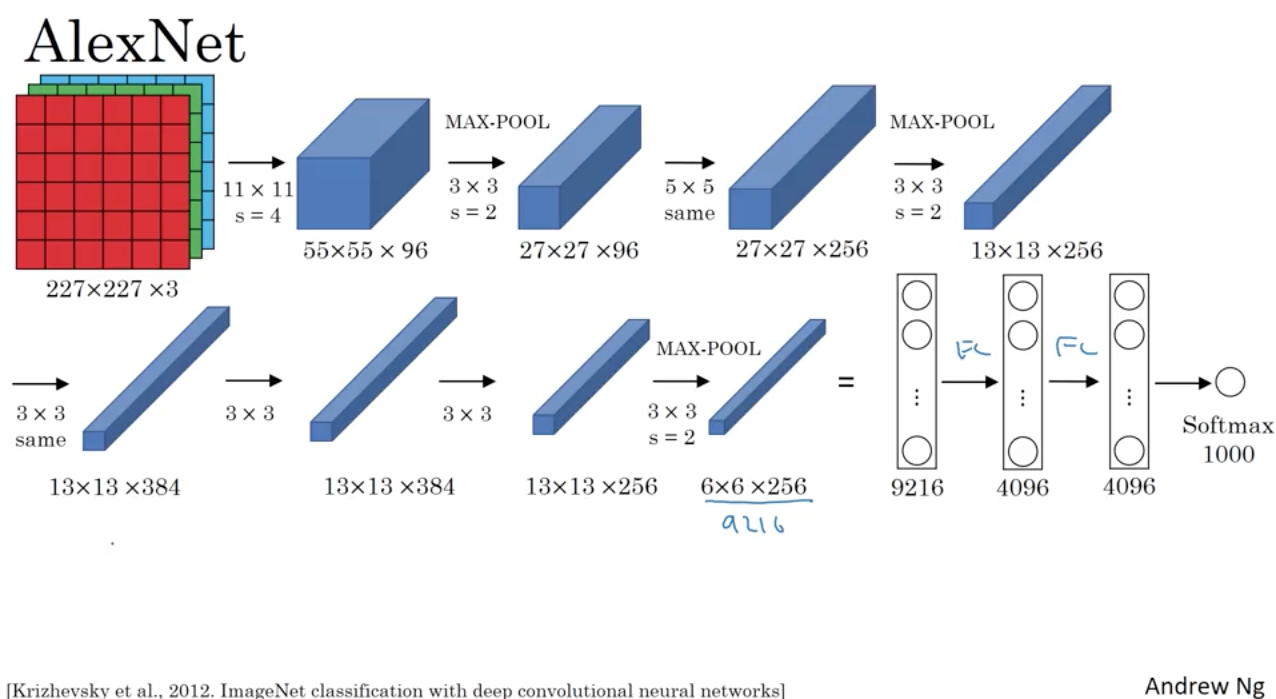
\includegraphics[width=1\columnwidth]{images/chap2/AlexNet.png}
  \caption{AlexNet Architecture}
  \label{chap2:WSP}
  \end{figure}
\end{center}
\textbf{GoogLeNet (Inception - 2014):} The ILSVRC 2014 winner was a Convolutional Network from Szegedy from Google. Its the main contribution was the development of an Inception Module that dramatically reduced the number of parameters in the network (4 million, compared to AlexNet with 60M). Besides that, Average Pooling instead of Fully Connected at the top layer of the model, eliminating a large number of parameters that do not seem to matter much.
\begin{center}
  \begin{figure}[H]
  \centering
  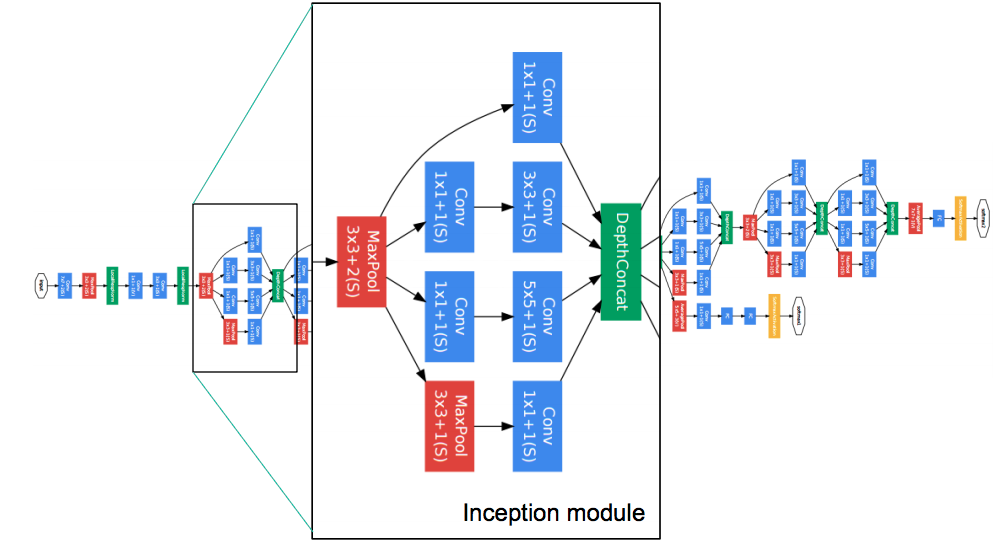
\includegraphics[width=1\columnwidth]{images/chap2/GoogleNet1.png}
  \caption{GoogleNet1 Architecture}
  \label{chap2:WSP}
  \end{figure}
\end{center}
\textbf{VGGNet (2014):} The runner-up in ILSVRC 2014 is invented by VGG (Visual Geometry Group) from the University of Oxford. Its main contribution was in showing that depth of the network is a critical component for good performance. 
\begin{center}
  \begin{figure}[H]
  \centering
  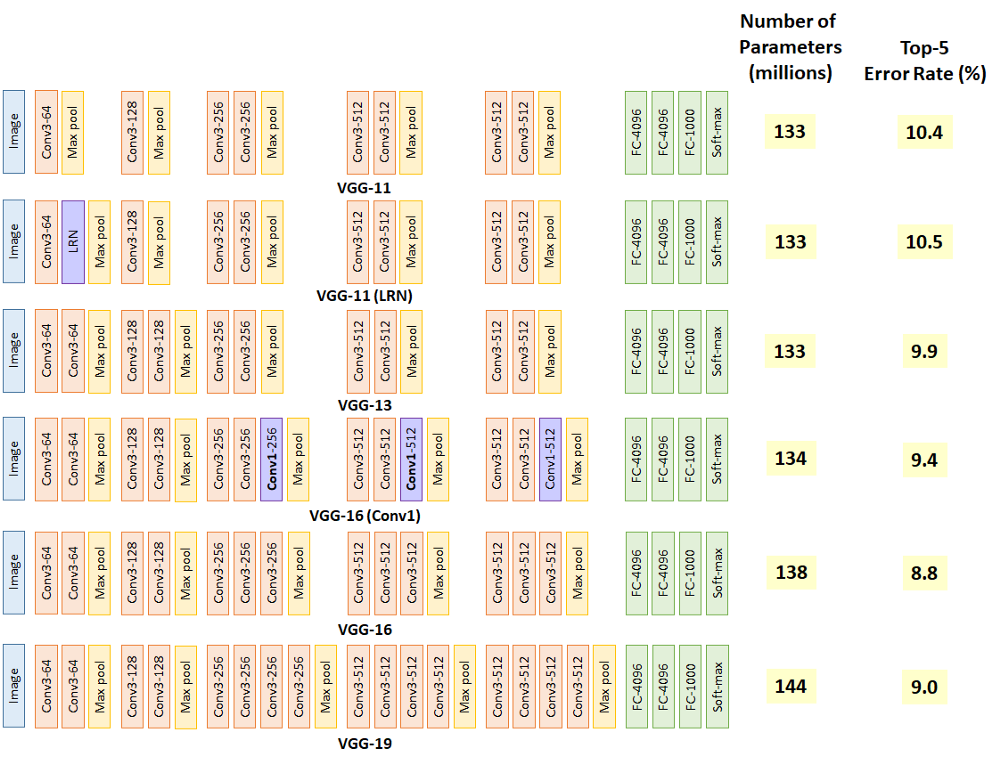
\includegraphics[width=1\columnwidth]{images/chap2/VGG_arch.png}
  \caption{VGG Architecture}
  \label{chap2:WSP}
  \end{figure}
\end{center}
\textbf{ResNet(2015):} at the ILSVRC 2015, the so-called Residual Neural Network (ResNet) by Kaiming He introduced architecture with “skip connections” and features heavy batch normalization. Such skip connections are also known as gated units or gated recurrent units and have a strong similarity to recent successful elements applied in RNNs, this technique able to train a Neural Network with 152 layers while still having lower complexity than VGGNet. It achieves a top-5 error rate of 3.57\% which beats human-level performance on this dataset.
\begin{center}
  \begin{figure}[H]
  \centering
  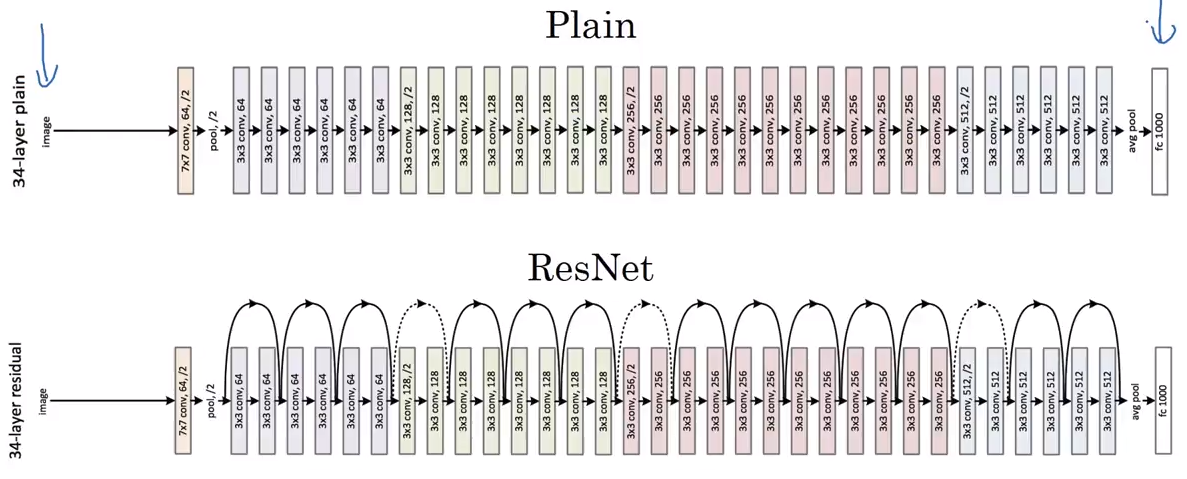
\includegraphics[width=1\columnwidth]{images/chap2/ResNet_Plain_Vs_Res.png}
  \caption{ResNet Architecture}
  \label{chap2:WSP}
  \end{figure}
\end{center}
\subsection{Recurrent Neural Network (RNN)}
Human understanding does not come from scratch for every new input. When a man is reading a paragraph, his understanding of each word is based on his knowledge of previous words. That is why a human brain is persistent.\\
Traditional neural networks cannot do the task above. For example, if a traditional network wants to classify a frame in a video, it cannot use its reasoning of previous frames to help with the result of the current frame.\\
\textbf{Recurrent Neural Networks (RNN)} fix this issue by having loops within them, thus allowing information to be persistent. The remaining of this section is about the basics of RNN and \textbf{Long Short-Term Memory Network (LSTM)}, a variation of RNN designed to avoid the long-term dependencies problem of RNNs.


\subsubsection{Recurrent Neural Network - RNN}
\textbf{Recurrent Neural Network} is a type of neural network effective for processing sequential data. Recurrent Neural Network (RNN) was first introduced by Rumelhart et al. In 1986 \cite{Rumelhart:1986:PDP:104279} as a family of neural networks suitable for processing of chain data. Unlike others neural networks, which can only handle input of a given size, RNN can handle any input of any length, and it is possible to model the dependency of the latter component. With preceding components in the output. First, the RNN stores a hidden state vector that is updated at each processing step (timestep) based on the value of this vector at the pre-processing stage and the value of the input component at this step. Second, the rules for hidden status updates, expressed through a set of corresponding functions and weights, are shared between processing steps. These features allow the RNN network to be generalizable even to any size input chain and have achieved the best results in processing string data such as text and sound.

Let x = $[x_{0}, x_{1}, ..., x_{n}]$ be an input sequence of $n + 1$ components with each component $x_{t}$ $(t = 0..n)$ is a vector of a certain size. Let $h_{t}$, $y_{t}$ denote the latent state and output of RNN in step t. An original RNN (Vanilla RNN) is represented by the following mathematical formula:
\begin{align}
h_{o} &= \sigma_{h}(W_{xh}x_{t})\\
h_{t} &= \sigma_{h}(W_{hh}h_{t-1} + W_{xh}x_{t})\\
y_{t} &= \sigma_{t}(W_{hy}h_{t})
\end{align}

In the above formula, $W_{hh}, W_{xh}$ and $W_{hy}$ are respectively the weight matrices between $h_{t-1}$ and $h_{t}, x_{t}$ and $h_{t}, h_{t}$ and $y_{t}$. $\sigma_{h}$ and $\sigma_{y}$ are activation functions, where the $\tanh$ function is usually used for $\sigma_{h}$.
\subsubsection{Long Short-Term Memory - LSTM}

\textbf{Long Short-Term Memory (LSTM)} was first introduced in 1997 by Hochreiter and Schmidhuber. LSTM is designed to handle Vanishing/Exploding Gradients problem through a method known as a gating mechanism. To understand what a gateway is, first look at how the LSTM works. Vector hidden state in LSTM network is calculated through the following formula:

\begin{align}
i &= \sigma ( W_{xi}x_{t} + W _{hi}h _{t-1} + b _{i}) \\
f &= \sigma(W_{xf}x_{t} + W_{hf}h_{t-1} + b_{f}) \\
o &= \sigma(W_{xo}x_{t} + W_{ho}h_{t-1} + b_{o})	\\
g &= \tanh (W_{xg}x_{t} + W_{hg}h_{t-1} + b_{g})	\\
c_{t} &= c_{t-1} \circ f+ g \circ I	\\
h_{t} &= \tanh(c_{t}) \circ o
\end{align}
\begin{center}
  \begin{figure}[H]
  \centering
  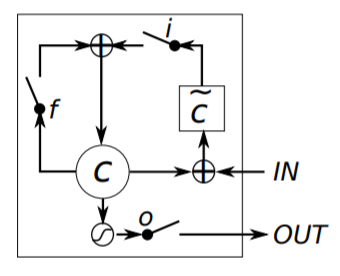
\includegraphics[width=0.5\columnwidth]{images/chap2/LSTM.png}
  \caption{Long Short-Term Memory cell \cite{DBLP:journals/corr/DonahueHGRVSD14}}
  \label{chap2:WSP}
  \end{figure}
\end{center}
In the above formulas:

$i$, $f$ and $o$ are respectively called \textbf{input gate}, \textbf{forget gate} and \textbf{output gate}. These gate have the same formula that is based on the input $x_{t}$ at the current step and the $h_{t-1}$ state of the previous step, but has different weighting matrices. These values are called $Gate$ because they have a trigger function of \textbf{Sigmoid} so that the value is always in the range [0, 1]. Moreover, by executing \textbf{Hadamard multiplication} (by multiplying the respective elements of the two matrices of the same size) between this and another vector of the same size, then determine the amount of information that this vector allows to pass through. The \textbf{input gate} specifies the amount of new information that is passed, this new information is calculated from the input component of the current step and the hidden state of the previous step. The \textbf{forget gate} specifies the amount of information the hidden state of the previous step is allowed to pass through. Finally, the \textbf{output gate} determines the amount of information from the inner state that is taken to the next step and the higher layers in the model. All ports are equal in size to the size of the hidden state vector.
\begin{center}
  \begin{figure}[H]
  \centering
  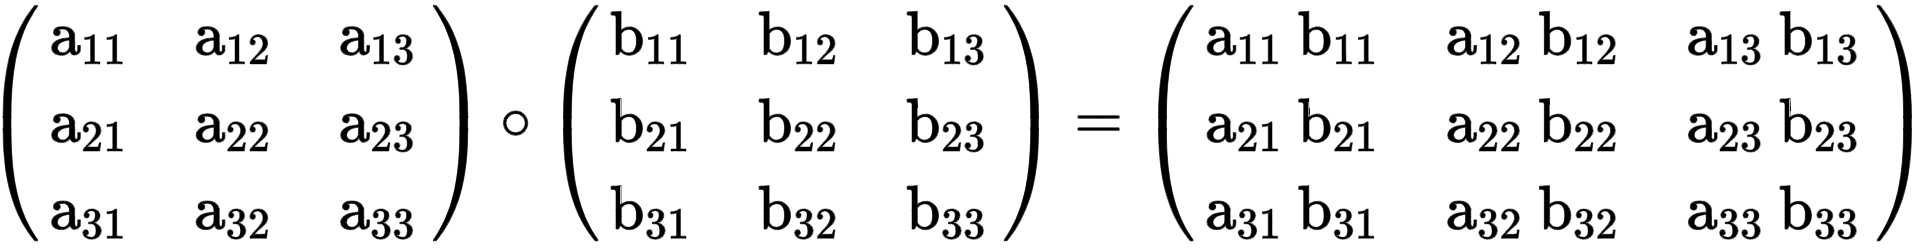
\includegraphics[width=0.8\columnwidth]{images/chap2/Hadamard.png}
  \caption{Hadamard multiplication}
  \label{chap2:WSP}
  \end{figure}
\end{center}

$g$ contains the combination of the hidden state of the previous step and the input component of the current step. In the pure RNN (Vanilla RNN), $g$ will be considered a new hidden state of the model. In the LSTM, the input gate will determine how much information from $g$ is used in the new hidden state.

$c_{t}$ is the internal memory of one unit. This is the memory combination between the memory value in the previous step $c_{t-1}$, multiplied by the \textbf{forget gate} and the value of $g$ multiplied by the input gate. So it can understand how internal memory is calculated by determining how much memory information is retained and how much information is added.

With the value of internal memory ($c_{t}$), it calculate the hidden state vector value by performing the \textbf{Hadamard multiplication} to the output gate ($o$) because not all of the internal memory values are related to the back-end layers, model or hidden state value of the next step



%\section{Face recognition}
%\section{Action recognition}
%\section{Cloud computing}
